Learning representations of inputs is the bedrock of all neural networks.

In recent years, Transformer models have been widely adapted to sequence modeling tasks in the vision and language domains, while Graph Neural Networks (GNNs) have been effective in constructing representations of nodes and edges in graph data. In the following questions we will explore both Transformers and GNNs, and draw some connections between them.

\textbf{Background:}

Let us first take a look at a graph model. We define a directed graph $G = \{V,E\}$ where $V$ is the set of all vertices and $E$ is the set of all edges. For $\forall v_i \in V$, let us define $\mathcal{N}(v_i)$ as the set of all of $v_i$'s neighbors with outgoing edges towards $v_i$. $v_i$ has a state representation $h_i^{t}$ at each time step $t$.

The values of $h_i^{t}$ are updated in parallel, using the same snapshot of the graph at a given time step. The procedures are as follows: We first need to aggregate the incoming data $H'_{it} = \{f_{ji}(h_j^{t})| \forall j, v_j \in \mathcal{N}(v_i)\}$ from neighbors using the function $Agg(H'_{it})$. Note that the incoming data from each neighbor is a transformed version of its representation using function $f_{ji}$. The aggregation function $Agg(H'_{it})$ can be something like the summation or the mean of elements in $H'_{it}$. 

Say the initial state at time step 0 is $h_i^{0}$. Now let us define the update rule for $h_i^{t}$ at time step $t+1$ as the following:
        \begin{equation} \label{eq:GNN}
            h_i^{t+1} = q(h_i^{t}, Agg(H'_{it}))
        \end{equation}
    where $q$ is a function - $Q_{t}: \{H_{t},Agg(H'_{t})\} \rightarrow H_{t}$, where $H_{t} = \{h_n^{t}| \forall n, v_n \in V\}$. 

Now, let us take a look at Transformer models. Recall that Transformer models build features for each word as a function of the features of all the other words with an attention mechanism over them, while RNNs update features in a sequential fashion. 

To represent a Transformer model's attention mechanism, let us define a feature representation $h_i$ for word $i$ in sentence $S$. We have the standard equation for the attention update at layer $l$ as a function of the each other word $j$ as follows:
\begin{align}
    h_{i}^{l+1} &= \texttt{Attention}(Q^{l}h^{l}_{i}, K^{l}h^{l}_{j}, V^{l}h^{l}_{j}) \label{eq: Attention1}\\
     &= \sum_{j\in S} \big( \texttt{softmax}_{j} (Q^{l}h^{l}_{i} \cdot K^{l}h^{l}_{j}) V^{l} h^{l}_{j} \big) \label{eq: Attention2}
\end{align}
where $Q^{l}, K^{l}, V^{l}$ are weight matrices for ``Query'', ``Key'', and ``Value''. $Q$ is a matrix that contains vector representations of one word in the sentence, while $K$ is a matrix containing representations for all the words in the sentence. $V$ is another matrix similar to $K$ that has representations for all words in the sentence. As a refresher for your knowledge about the Transformer model, you can refer to this \href{https://arxiv.org/abs/1706.03762}{paper}.


Based on the above background information, answer the following questions:

\begin{enumerate}
    \item 
    
    If the aggregation operation for $Agg(H'_{it})$ is the summation of representation of all adjacent vertices, rewrite the equation \ref{eq:GNN} by replacing $Agg(H'_{it}))$ in terms of $\mathcal{N}$, $f$, and $h$.
    
    \item Consider the directed graph G in Fig~\ref{fig: graph}.
    \begin{figure}[h] 
        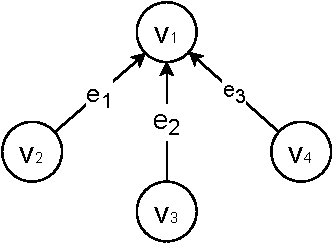
\includegraphics[scale = 0.8]{assets/graph.pdf}
        \centering
        \caption{}\label{fig: graph}
    \end{figure}
    The values for the vertices at time step t are as follows:
    \begin{equation}
        h_1^{t} = [1, -1] \quad h_2^{t} = [-1, 1] \quad h_3^{t} = [0, -1]\quad h_4^{t} = [1, 0]
    \end{equation}
    
    The aggregation function $Agg(H'_{1t})$ is:
    \begin{equation}
        Agg(H'_{1t}) = [0.6, 0.2, 0.2] \begin{bmatrix}
           f(h_{2}^{t}) \\
           f(h_{3}^{t}) \\
           f(h_{4}^{t})
         \end{bmatrix}
    \end{equation}
    
   And the function $f$ on all the edges is:
    \begin{equation}
        f(x) = 2x
    \end{equation}
    
    Now, given that
    \begin{equation}
        h_1^{t+1} = q(h_1^{t}, Agg(H'_{1t})) = W(h_1^{t})^{T} + max\{Agg(H'_{1t}),0\}
    \end{equation}where $W = [1,1]$, what is the updated value of $h_1^{t+1}$?
\end{enumerate}

\begin{enumerate}[resume]
    \item Consider the graph G in question (b). We want to alter it to represent the sentence "I eat red apples" (4 word tokens) as a fully connected graph. Each vertex represents one word token, and the edges represent the relationships among the tokens. How many edges in all would graph G contain? Notice that the edges are directed and a bi-directional edge counts as two edges.
    \item Using equations \ref{eq:GNN} and \ref{eq: Attention2}, show that the Transformer model's single-head attention mechanism is equivalent to a special case of a GNN. 
    \item An ongoing area of research in Transformer models for NLP is the challenge of learning very-long-term dependencies among entities in a sequence. Based on this connection with GNNs, why do you think this could be problematic? 
\end{enumerate}
